\lecture{绪论}{lec:chap01}
\section[基本特性]{对象、类及其特性}\label{sec:chap01-sec01}
%%%%%%%%%%%%%%%%%%%%%%%%%%%%%% 对象、类及其特性 %%%%%%%%%%%%%%%%%%%%%%%%%%%%%%%%%%
\begin{frame}{基本特性}{普通定义}
  \stretchon
  \begin{itemize}
  \item 对象
    \begin{itemize}
    \item 目标
    \item 恋爱的对方
    \item 描写或写实的人或物
    \end{itemize}
  \item Object
    \begin{itemize}
    \item Something perceptible by one or more of the senses,
      especially by vision or touch; a material thing
    \item The purpose or goal of a specific action
    \item \ldots\ldots
    \end{itemize}
  \end{itemize}
  \stretchoff
\end{frame}

\begin{frame}{基本特性}{课程定义}
  \stretchon
  \begin{itemize}
  \item 对象(现实世界)
    \begin{itemize}
    \item 现实世界中的某个具体的事物(实物或实体)
    \item 一个封装了属性(attribute)与行为(behavior)的实体
    \end{itemize}
  \item 对象(计算机世界)---\alert{数据结构}
    \begin{itemize}
    \item 数据域
    \item 方法
    \item 相互作用关系
    \end{itemize}
  \end{itemize}
  \stretchoff
\end{frame}

\begin{frame}{基本特性}{对象实例:树}
  \stretchon
  \begin{itemize}
  \item 属性
    \begin{itemize}
    \item 树干树枝、树叶、树龄、纹理、荷尔蒙\ldots\ldots
    \end{itemize}
  \end{itemize}
  \centering
  %\begin{center}
    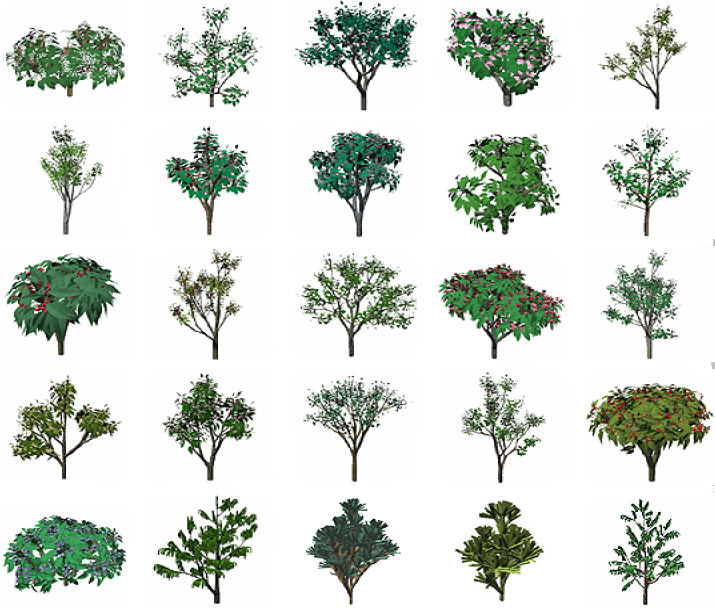
\includegraphics[height=0.6\textheight]{chap01/01trees} %
    % \end{center}
  \stretchoff
\end{frame}

\begin{frame}{基本特性}{对象实例:树}
  \stretchon
  \begin{itemize}
  \item 方法(行为、操作)
    \begin{itemize}
    \item 生长、四季变化、修剪、运动、叶枝摩擦、声音\ldots\ldots
    \end{itemize}
  \end{itemize}
  \vspace{-1ex}
  \centering
  %\begin{center}
    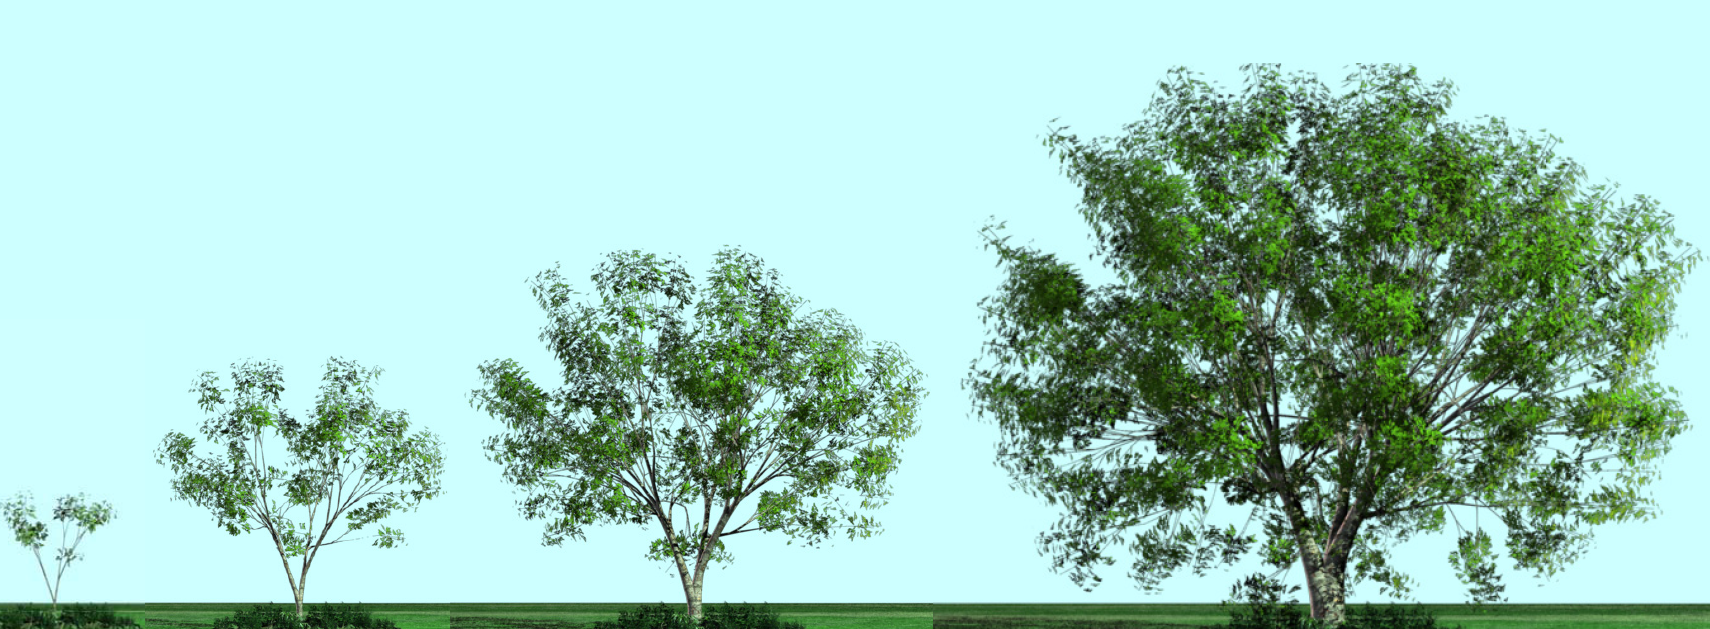
\includegraphics[height=0.25\textheight]{chap01/02treesgrow} \\[1ex]%
    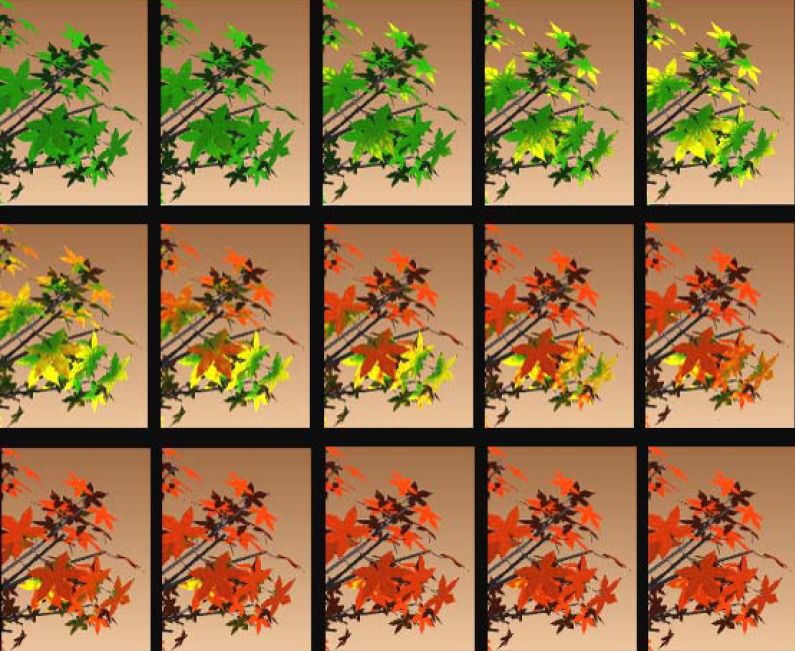
\includegraphics[height=0.45\textheight]{chap01/03treesseason} %
  %\end{center}
  \stretchoff
\end{frame}

\begin{frame}{基本特性}{对象实例:俄罗斯方块}
  \stretchon
  \begin{itemize}
  \item 属性
    \begin{itemize}
    \item 颜色,四个方块的布局,大小,位置,速度,\ldots\ldots
    \end{itemize}
  \item 行为
    \begin{itemize}
    \item 平移,旋转,加速,碰撞检测,显示,\ldots\ldots
    \end{itemize}
  \end{itemize}
  \centering
  %\begin{center}
    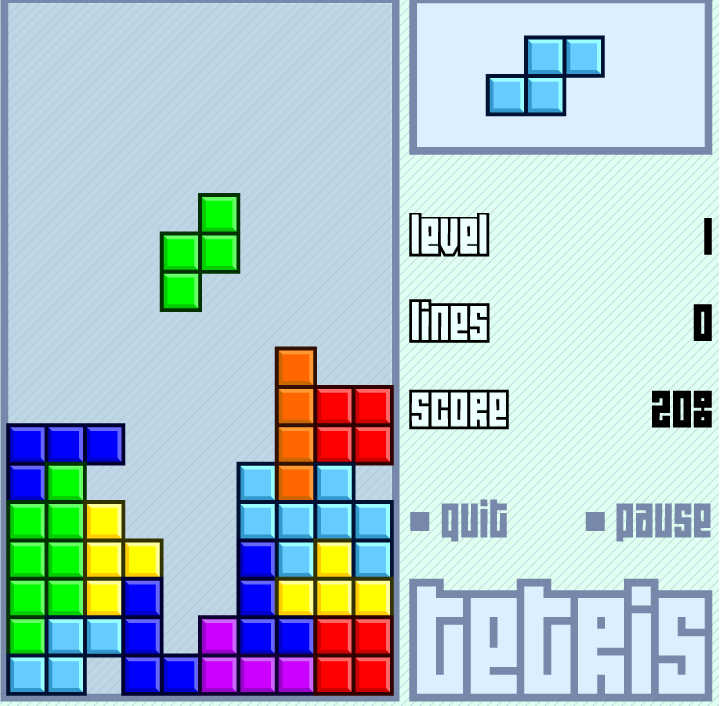
\includegraphics[width=0.35\textwidth]{chap01/04tetrogame} \qquad%
    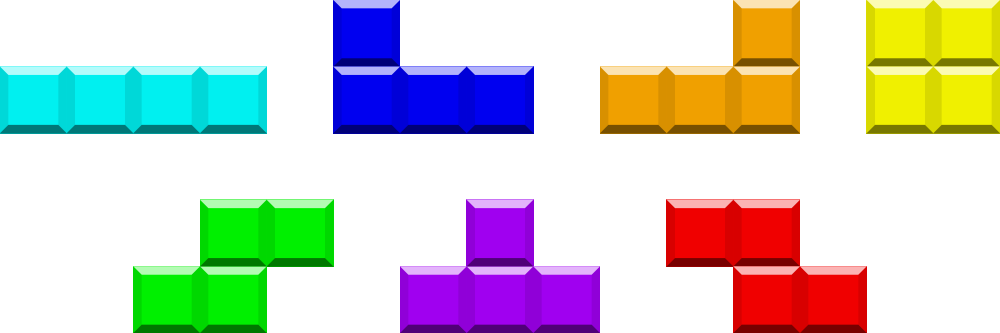
\includegraphics[width=0.55\textwidth]{chap01/05tetroobj} %
  %\end{center}
  \stretchoff
\end{frame}

\begin{frame}[t, fragile]{基本特性}{消息(message)}
  \begin{itemize}
  \item 类\\
    \begin{minipage}{0.8\linewidth}
      \begin{cpptt}
CTetromino{
  |\textbf{\textcolor{blue}{属性:}}颜色,四个方块的布局,大小,位置,速度,$\cdots$|
  |\textbf{\textcolor{blue}{行为:}}平移,旋转,加速,碰撞检测,显示,$\cdots$|
};
      \end{cpptt}
    \end{minipage}
  \item 类对象\\
    \begin{minipage}{0.8\linewidth}
      \begin{cppcode}
CTetromino I, J, L, O, S, T, Z;
      \end{cppcode}
    \end{minipage}
  \item 操作对象
    \begin{itemize}
    \item 向对象发送消息
    \item 通过调用对象的操作实现
    \end{itemize}
    \begin{minipage}{0.5\linewidth}
      \begin{cpptt}
CTetromino S(|\textcolor{green}{绿色}|, 01101100);
S.|平移|(-1, 0);
      \end{cpptt}
    \end{minipage} \qquad
    \onslide<2->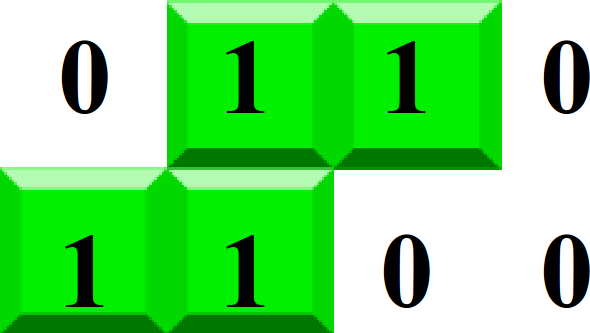
\includegraphics[width=0.12\textwidth]{chap01/06tetromove}\qquad%
    \onslide<1>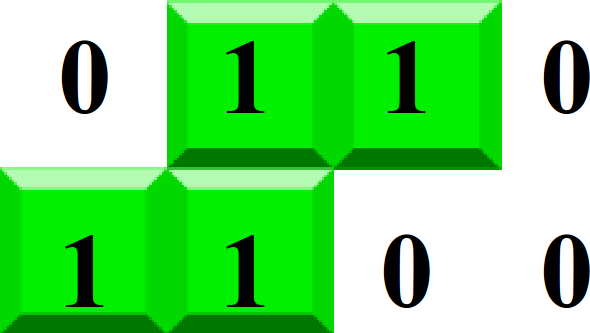
\includegraphics[width=0.12\textwidth]{chap01/06tetromove}%
  \end{itemize}
\end{frame}

\begin{frame}{基本特性}{数据抽象(Data abstraction)}
  \stretchon
  \begin{itemize}
  \item 抽象
    \begin{itemize}
    \item 抽取共性
    \item 问题空间的事物 $\Rightarrow$ 解空间的面向对象的概念
    \end{itemize}
  \item 示例1:两栖动物\\
    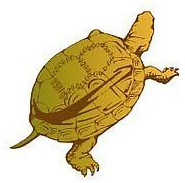
\includegraphics[width=0.2\textwidth]{chap01/07abstraction01} \qquad%
    
\includegraphics[width=0.2\textwidth]{chap01/07abstraction02} \qquad%
    
\includegraphics[width=0.2\textwidth]{chap01/07abstraction03} %
  \item 示例2:斑马\\
    \centering
    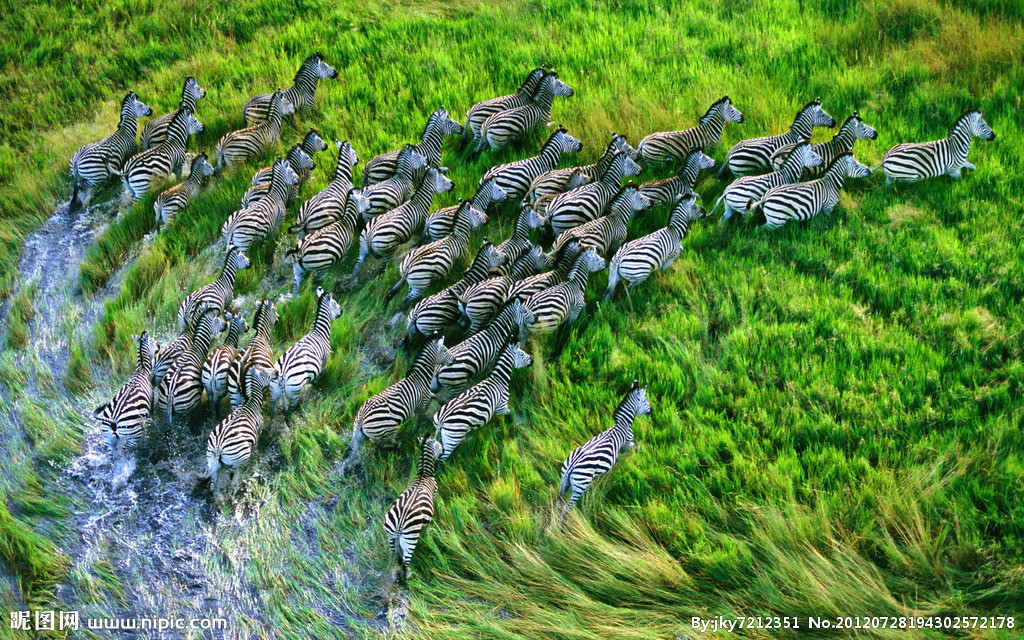
\includegraphics[width=0.3\textwidth]{chap01/07abstraction04}    
  \end{itemize}
  \stretchoff
\end{frame}

\begin{frame}{基本特性}{封装性(Encapsulation)}
  \stretchon
  \begin{itemize}
  \item 对象的\alert{属性}和\alert{服务}结合成一个\alert{独立的系统单
      位}
  \item 隐蔽对象的\alert{内部细节}
  \item 保留有限的\alert{对外接口}
  \item \alert{代码安全性}
  \item 示例:\\
    \centering
    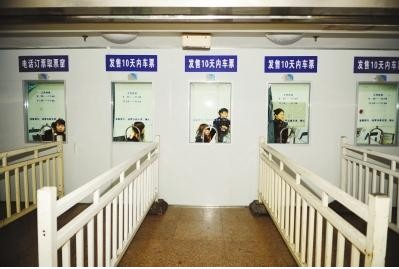
\includegraphics[width=0.4\textwidth]{chap01/08encap01}\qquad%
    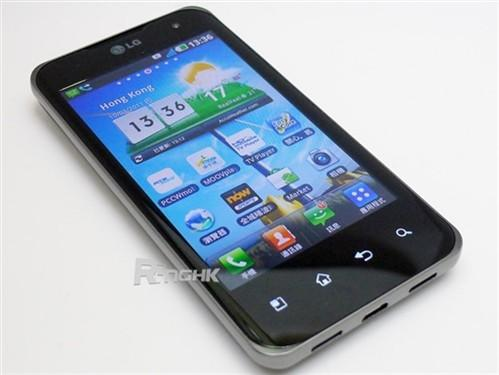
\includegraphics[width=0.4\textwidth]{chap01/08encap02}
  \end{itemize}
  \stretchoff
\end{frame}

\begin{frame}{基本特性}{类和对象的UML图示}
  \begin{columns}[c]
    \begin{column}{0.4\textwidth}
      \begin{spacing}{1.5}
      \begin{itemize}
      \item 类(三栏矩形)
        \begin{itemize}
        \item 类名
        \item 属性
        \item 操作
        \item 对外可见性
          \begin{itemize}
          \item ``+''---公有
          \item ``-''---私有
          \end{itemize}
        \end{itemize}
      \item 对象(矩形)
        \begin{itemize}
        \item 对象名称
        \item 类型
        \item 属性值
        \end{itemize}
      \end{itemize}
      \end{spacing}
    \end{column}
    \begin{column}{0.6\textwidth}
      \tiny
      \centering
      \begin{tikzpicture}
        \begin{class}[text width=0.2\textwidth]{类名}{0, 0}
          \attribute{- 属性1}
          \attribute{- 属性2}

          \operation{+ 操作1()}
          \operation{+ 操作2()}
        \end{class}
        
        \begin{class}[text width=0.7\textwidth]{Circle}{0, -3}
          \attribute{- radius : double}
          \attribute{- center\_x : int}
          \attribute{- center\_y : int}
          
          \operation{+ area() : double}
          \operation{+ perimeter() : double}
          \operation{+ move(in newx : int, in newy : int) : void}
          \operation{+ scale(in factor : double) : void}
        \end{class}
      \end{tikzpicture}
    \end{column}
  \end{columns}
\end{frame}

\begin{frame}{基本特性}{类和对象的UML图示}
  \begin{columns}[c]
    \begin{column}{0.4\textwidth}
      \begin{spacing}{1.5}
      \begin{itemize}
      \item 类(三栏矩形)
        \begin{itemize}
        \item 类名
        \item 属性
        \item 操作
        \item 对外可见性
          \begin{itemize}
          \item ``+''---公有
          \item ``-''---私有
          \end{itemize}
        \end{itemize}
      \item 对象(矩形)
        \begin{itemize}
        \item 对象名称
        \item 类型
        \item 属性值
        \end{itemize}
      \end{itemize}
      \end{spacing}
    \end{column}
    \begin{column}{0.6\textwidth}
      \tiny
      \centering
      \begin{tikzpicture}
        \begin{class}[text width=0.2\textwidth]{类名}{0, 0}
          \operation{+ 操作1()}
          \operation{+ 操作2()}
        \end{class}
        
        \begin{class}[text width=0.7\textwidth]{Circle}{0, -3}
          \operation{+ area() : double}
          \operation{+ perimeter() : double}
          \operation{+ move(in newx : int, in newy : int) : void}
          \operation{+ scale(in factor : double) : void}
        \end{class}
      \end{tikzpicture}
    \end{column}
  \end{columns}
\end{frame}

\begin{frame}{基本特性}{类和对象的UML图示}
  \begin{columns}[c]
    \begin{column}{0.4\textwidth}
      \begin{spacing}{1.5}
      \begin{itemize}
      \item 类(三栏矩形)
        \begin{itemize}
        \item 类名
        \item 属性
        \item 操作
        \item 对外可见性
          \begin{itemize}
          \item ``+''---公有
          \item ``-''---私有
          \end{itemize}
        \end{itemize}
      \item 对象(矩形)
        \begin{itemize}
        \item 对象名称
        \item 类型
        \item 属性值
        \end{itemize}
      \end{itemize}
      \end{spacing}
    \end{column}
    \begin{column}{0.6\textwidth}
      \tiny
      \centering
      \begin{tikzpicture}
        \begin{class}[text width=0.2\textwidth]{类名}{0, 0}          
        \end{class}        
        \begin{class}[text width=0.2\textwidth]{Circle}{3, 0}          
        \end{class}
      
        \begin{object}[text width=0.3\textwidth]{对象名称}{0, -3}
          \instanceOf{类名}
          \attribute{属性1=值1}
          \attribute{属性2=值2}
        \end{object}

        \begin{object}[text width=0.4\textwidth]{cobj}{3, -3}
          \instanceOf{Circle}
          \attribute{radius : double = 2.7}
          \attribute{center\_x : int = 10}
          \attribute{center\_y : int = 20}
        \end{object}
      \end{tikzpicture}
    \end{column}
  \end{columns}
\end{frame}

\begin{frame}{基本特性}{继承性(Inheritance)}
  \stretchon
  \begin{itemize}
  \item 一般类 $\Rightarrow$ 特殊类(\alert{具备全部属性与行为})
  \item \alert{代码重用}
  \item 示例1:\\
    \centering
    \scalebox{0.5}{
    \begin{tikzpicture}
      \path[mindmap, text=white,%concept color=black,text=white]
               root concept/.append style={concept color=black},
               level 1 concept/.append style={level distance=60, sibling angle=90}
           ]
      node[concept]{马}
      [clockwise from=-45]
      child[concept color=green!50!black] {
        node[concept] {蒙古马}
      }
      child[concept color=blue] {
        node[concept] {斑马}
      };
    \end{tikzpicture}
    }\\
    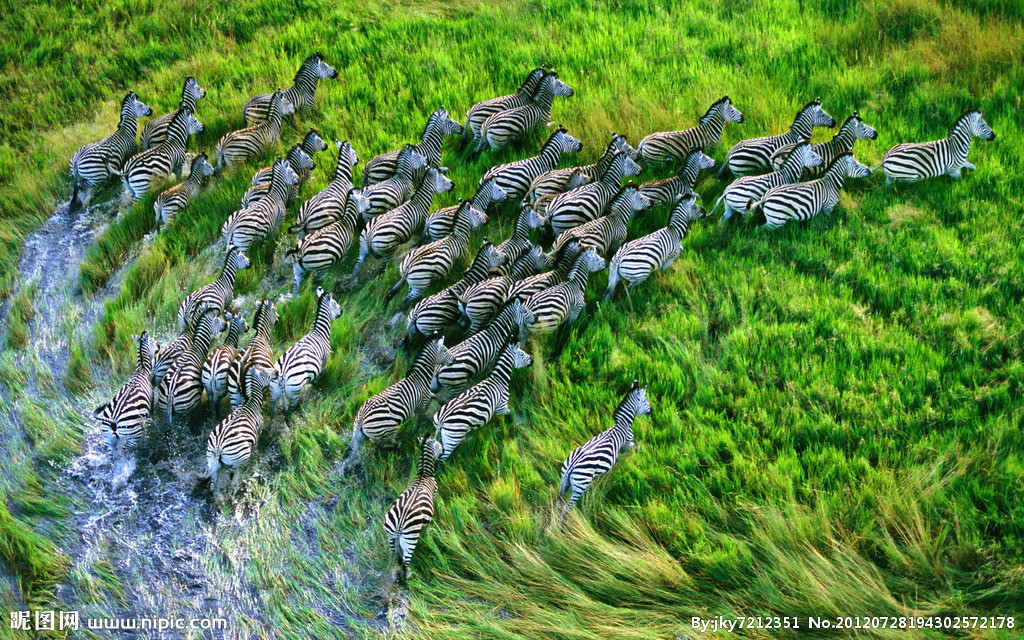
\includegraphics[width=0.4\textwidth]{chap01/09inherit01}\qquad%
    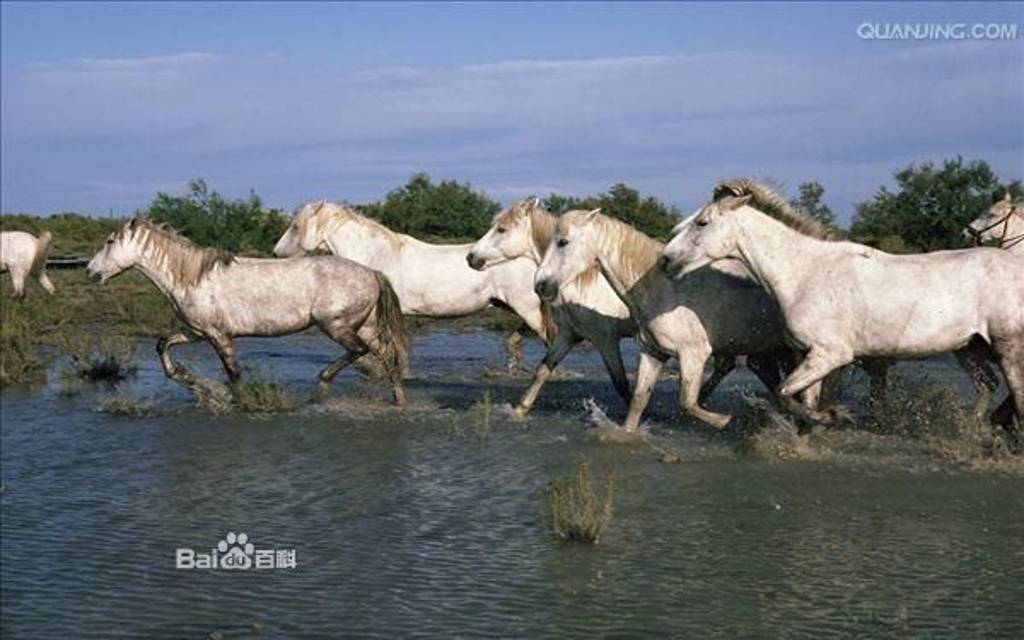
\includegraphics[width=0.4\textwidth]{chap01/09inherit02}
  \end{itemize}
  \stretchoff
\end{frame}

\begin{frame}[fragile]{基本特性}{继承性(Inheritance)}
  \begin{itemize}
  \item 示例2(伪代码):\\
    \begin{minipage}{0.8\linewidth}
      \begin{cpptt}
Animal|类|{
    Animal|类|(const string& name) : name(name) {}
    virtual string talk() = 0;
    const string name;
};
      \end{cpptt}
    \end{minipage}\\
    \begin{minipage}{0.8\linewidth}
      \begin{cpptt}
Cat|类| : Animal|类|{
    Cat|类|(const string& name): Animal|类|(name) {}
    string talk() { return "喵喵!"; }
};
      \end{cpptt}
    \end{minipage}
    \begin{minipage}{0.8\linewidth}
      \begin{cpptt}
Dog|类| : Animal|类|{
    Dog|类|(const string& name): Animal|类|(name) {}
    string talk() { return "汪汪!"; }
};
      \end{cpptt}
    \end{minipage}  
  \end{itemize}
\end{frame}

\begin{frame}{基本特性}{继承性(Inheritance)}
  \stretchon
  \begin{itemize}
  \item 类的继承
  \end{itemize}
  %\stretchon
  \tiny
  %\centering
  \qquad\qquad\qquad\qquad
  \begin{tikzpicture}
    \begin{class}[text width=0.2\textwidth]{父类}{0, 0}
      \operation{+ 操作1()}
      \operation{+ 操作2()}
    \end{class}
    \begin{class}[text width=0.2\textwidth]{子类1}{-2, -1.5}
      \inherit{父类}
      \operation{+ 操作3()}
    \end{class}
    \begin{class}[text width=0.2\textwidth]{子类2}{2, -1.5}
      \inherit{父类}
      \operation{+ 操作4()}
    \end{class}
  
    \begin{class}[text width=0.2\textwidth]{A}{-2, -3}
      \operation{+ 操作1()} \operation{+ 操作2()}
    \end{class}
    \begin{class}[text width=0.2\textwidth]{B}{-2, -4.5}
      \inherit{A}
      % \operation{+ 操作3()}
    \end{class}

    \begin{class}[text width=0.2\textwidth]{Rectangle}{2, -3}
      \attribute{- width}
      \attribute{- length}
      \operation{+ area()}
      \operation{+ perimeter()}
      \operation{+ scale()}
    \end{class}
    \begin{class}[text width=0.2\textwidth]{Square}{2, -5.3}
      \inherit{Rectangle}
      \operation{+ scale()}
    \end{class}
  \end{tikzpicture}
  \stretchoff
\end{frame}

\begin{frame}{基本特性}{继承性(Inheritance)}
  \stretchon
  \begin{itemize}
  \item 类的继承
  \end{itemize}
  \tiny
  \centering
  %\qquad\qquad\qquad\qquad\qquad\qquad
  \begin{tikzpicture}
    \begin{class}[text width=0.2\textwidth]{电话机}{0, 0}
      \operation{+ 拨出()}
      \operation{+ 接听()}
    \end{class}
    
    \begin{class}[text width=0.2\textwidth]{固定话机}{-2, -1.5}
      \inherit{电话机}
      %\operation{+ 操作3()}
    \end{class}
    
    \begin{class}[text width=0.2\textwidth]{手机}{2, -1.5}
      \inherit{电话机}
      \operation{+ 发送短信()}
      \operation{+ 接收短信()}
    \end{class}

    \begin{class}[text width=0.2\textwidth]{音乐手机}{0, -3.5}
      \inherit{手机}
      \operation{+ 播放音乐()}
    \end{class}
    
    \begin{class}[text width=0.2\textwidth]{3G手机}{4, -3.5}
      \inherit{手机}
      \operation{+ 网络电视()}
      \operation{+ 收发电邮()}
    \end{class}  
    
  \end{tikzpicture}
  \stretchoff
\end{frame}

\begin{frame}[fragile]{基本特性}{多态性(Polymorphism)}
  %\stretchon
  \begin{itemize}
  \item 在\alert{一般类}中定义的属性或行为,被\alert{特殊类继承}之后,
    可以具有不同的数据类型或表现出\alert{不同的行为}\\
    \begin{minipage}{0.8\linewidth}
      \begin{cpptt}
Animal|类| *animalCat = new Cat|类|("爱丽丝");
Animal|类| *animalDog = new Dog|类|("旺财");

cout << animalCat->name << ": " << animalCat->talk() << endl;
cout << animalDog->name << ": " << animalDog->talk() << endl;
      \end{cpptt}
    \end{minipage}
  \end{itemize}
  
  \begin{center}
    \begin{tikzpicture}[font=\scriptsize]
      \begin{class}[text width=0.2\textwidth]{Animal}{0, 0}
        \attribute{- name}
        \operation{+ talk()}
      \end{class}
    
    \begin{class}[text width=0.2\textwidth]{Cat}{-2, -2.5}
      \inherit{Animal}
      \attribute{- name}
      \operation{+ talk()}
    \end{class}
    
    \begin{class}[text width=0.2\textwidth]{Dog}{2, -2.5}
      \inherit{Animal}
      \attribute{- name}
      \operation{+ talk()}
    \end{class}
  \end{tikzpicture}
\end{center}
  %\stretchoff
\end{frame}

\begin{frame}{基本特性}{多态性(Polymorphism)}
  \stretchon
  \begin{itemize}
  \item 形状类
  \end{itemize}  
  \centering%begin{center}
    \begin{tikzpicture}[font=\scriptsize]
      \begin{class}[text width=0.2\textwidth]{shape}{0, 0}
        \attribute{-center}        
        \operation{+area()}
        \operation{+perimeter()}
        \operation{+draw()}
        \operation{+erase()}
      \end{class}
    
    \begin{class}[text width=0.2\textwidth]{circle}{-3.5, -3.5}
      \inherit{shape}
      \attribute{-radius}
      \operation{+area()}
      \operation{+perimeter()}
    \end{class}
    
    \begin{class}[text width=0.2\textwidth]{rectangle}{0, -3.5}
      \inherit{shape}
      \attribute{-width}
      \attribute{-height}
      \operation{+area()}
      \operation{+perimeter()}
    \end{class}

    \begin{class}[text width=0.2\textwidth]{triangle}{3.5, -3.5}
      \inherit{shape}
      \attribute{-a}
      \attribute{-b}
      \attribute{-c}
      \operation{+area()}
      \operation{+perimeter()}
    \end{class}
  \end{tikzpicture}
%\end{center}
  \stretchoff
\end{frame}

\begin{frame}{基本特性}{类之间的关系}
  %\stretchon
  \begin{itemize}
  \item 组合
    \begin{itemize}
    \item 整体和部分关系
    \item 同时存在
    \item 同时销毁
    \end{itemize}
  \end{itemize}
  \vspace{4ex}
  \centering%begin{center}
  \begin{tikzpicture}[font=\scriptsize]
    \begin{class}[text width=0.1\textwidth]{计算机}{0, 0}
    \end{class}

    \begin{class}[text width=0.1\textwidth]{显示器}{3, 0}
    \end{class}

    \begin{class}[text width=0.1\textwidth]{主机}{-3, 0}
    \end{class}

    \begin{class}[text width=0.1\textwidth]{键盘}{-2, -2.5}
    \end{class}

    \begin{class}[text width=0.1\textwidth]{鼠标}{2, -2.5}
    \end{class}
    
    \composition{计算机}{}{1..*}{显示器}
    \composition{计算机}{}{1}{主机}
    \composition{计算机}{}{0..1}{鼠标}
    \composition{计算机}{}{1}{键盘}
  \end{tikzpicture}
  %\stretchoff
\end{frame}

\begin{frame}{基本特性}{类之间的关系}
  %\stretchon
  \begin{itemize}
  \item 聚合
    \begin{itemize}
    \item 包含关系
    \item 共享成员
    \item \alert{组合的泛化}
    \end{itemize}
  \end{itemize}
  \vspace{4ex}
  \centering%begin{center}
  \begin{tikzpicture}[font=\scriptsize]
    \begin{class}[text width=0.1\textwidth]{球队}{0, 0}
    \end{class}

    \begin{class}[text width=0.1\textwidth]{球员}{4, 0}
    \end{class}

    \begin{class}[text width=0.1\textwidth]{主教练}{4, -2.5}
    \end{class}
    
    \aggregation{球队}{}{*}{球员}
    \aggregation{球队}{}{1}{主教练}
  \end{tikzpicture}
  %\stretchoff
\end{frame}

\begin{frame}{基本特性}{类之间的关系}
  %\stretchon
  \begin{itemize}
  \item 关联
    \begin{itemize}
    \item 消息传递链
    \item \alert{聚合的泛化}
    \end{itemize}
  \end{itemize}
  \vspace{6ex}
  \centering%begin{center}
  \begin{tikzpicture}[font=\scriptsize]
    \begin{class}[text width=0.1\textwidth]{公司}{0, 0}
    \end{class}

    \begin{class}[text width=0.1\textwidth]{员工}{6, 0}
    \end{class}
    
    \association[工作]{公司}{雇主}{0..1}{员工}{1..*}{雇员}
  \end{tikzpicture}
  %\stretchoff
\end{frame}

\begin{frame}{基本特性}{类之间的关系}
  %\stretchon
  \begin{itemize}
  \item 依赖
    \begin{itemize}
    \item 短时使用关系
    \item \alert{非永久关系}
    \end{itemize}
  \end{itemize}
  \vspace{6ex}
  \centering%begin{center}
  \begin{tikzpicture}[font=\scriptsize]
    \begin{class}[text width=0.1\textwidth]{Word文档}{0, 0}
    \end{class}

    \begin{class}[text width=0.2\textwidth]{打印机}{4, 0}
      \operation{+打印()}
    \end{class}
    
    \unidirectionalAssociation{Word文档}{}{}{打印机}
  \end{tikzpicture}
  %\stretchoff
\end{frame}



%%%%%%%%%%%%%%%%%%%%%%%%%%%%%%%%%%%%%%%%%%%%%%%%%%%%%%%%%%%%%%%%%%%%%%%%%%

\section[是什么?]{什么是面向对象程序设计}\label{sec:chap01-sec02}
%%%%%%%%%%%%%%%%%%%%%%%%%%%%%% 什么是面向对象程序设计 %%%%%%%%%%%%%%%%%%%%%%%%%%%%%%%
\begin{frame}{是什么?}{什么是面向对象程序设计}
  \stretchon
  \begin{itemize}
  \item 使用\alert{对象}去设计程序编写代码的一种方法
    \begin{itemize}
    \item 数据抽象
    \item 信息隐藏
    \item 代码重用
    \end{itemize}
  \end{itemize}
  
  \centering
  \begin{tikzpicture}[node distance=2.5cm, auto, >=stealth]
    % nodes
    \node[block] (ooa) {Analysis(OOA)};
    \node[block] (ood) [right of=ooa,below of=ooa, node
    distance=1cm] {Design(OOD)};
    \node[block] (oop) [right of=ood,below of=ood, node distance=1cm]
    {Programming(OOP)};
    \node[block] (oot) [right of=oop,below of=oop, node
    distance=1cm] {Test(OOT)};        
    \node[block] (oom) [right of=oot,below of=oot, node
    distance=1cm] {Maintenance(OOM)};

    \draw[->] (ooa) -- (ood);
    \draw[->] (ood) -- (ooa);
        
    \draw[->] (ood) -- (oop);
    \draw[->] (oop) -- (ood);

    \draw[->] (oop) -- (oot);
    \draw[->] (oot) -- (oop);

    \draw[->] (oot) -- (oom);
    \draw[->] (oot) -- (oom);

    \draw[->] (oop.east) to  [out=0,in=0] (ooa.east);
        
    \draw[->] (oot.west)  to  [out=180,in=180] (ood.west);
  \end{tikzpicture}
  \stretchoff
\end{frame}
%%%%%%%%%%%%%%%%%%%%%%%%%%%%%%%%%%%%%%%%%%%%%%%%%%%%%%%%%%%%%%%%%%%%%%%%%%

\section[为什么?]{为何学习面向对象程序设计}\label{sec:chap01-sec03}
%%%%%%%%%%%%%%%%%%%%%%%%%%%%% 为何学习面向对象程序设计 %%%%%%%%%%%%%%%%%%%%%%%%%%%%%%
\begin{frame}{为什么?}{为何学习面向对象程序设计}
  \stretchon
  \begin{itemize}
  \item 过程式程序设计
    \begin{itemize}
    \item 数据和过程分离,可维护性与可重用性差
    \item 不适于大型程序开发
    \end{itemize}
  \item 面向对象程序设计
    \begin{itemize}
    \item 现实世界的直接模拟
    \item 可重用性好,可维护性好
    \item 适合大型程序开发
    \end{itemize}
  \end{itemize}
  \stretchoff
\end{frame}
%%%%%%%%%%%%%%%%%%%%%%%%%%%%%%%%%%%%%%%%%%%%%%%%%%%%%%%%%%%%%%%%%%%%%%%%%%

\section[发展史]{面向对象程序设计语言发展史}\label{sec:chap01-sec04}
%%%%%%%%%%%%%%%%%%%%%%%%%%%% 面向对象程序设计语言发展史 %%%%%%%%%%%%%%%%%%%%%%%%%%%%%%
\begin{frame}[fragile]{发展史}{族谱}
  \stretchon
  \begin{itemize}
  \item 族谱(Family tree)    
  \end{itemize}
  \centering
  \scalebox{0.7}{
  \tikzset{box/.style={rectangle, draw=black, rounded corners}}
  \tikzset{boxgreen/.style={rectangle, draw=black, rounded corners,fill=green}} 
  \begin{tikzpicture}%[scale=\s, every node/.style={scale=\s}]
    \node[box] (asm) {Assembler};
    \node[box] (for) [right=0.5 of asm] {Fortran};
    \node[box] (alg)  [right=0.5  of for] {Algol};
    \node[box] (bcp)  [right=0.5  of alg] {BCPL};
    \node[box] (pas)  [above=1  of bcp] {Pascal};
    \node[boxgreen] (sim) [below=1 of bcp] {Simula};
    \node[box] (c) [right=0.5 of bcp] {C};
    \node[box] (cpp) [right=0.5 of c] {C++};
    \node[box] (cpp0x) [right=0.5 of cpp] {C++0x};
    \node[box] (opas) [above=1 of cpp0x, right=3.1 of pas] {Object Pascal};
    \node[boxgreen] (lisp) [below=2.5 of alg] {Lisp};
    \node[boxgreen] (smt) [right=2.5 of lisp] {Smalltalk};
    \node[box] (jar) [below=2.5 of cpp0x, right=0.8 of smt] {Java};
    \node (endmain)  [right=0.5  of cpp0x] {};
    \node (endopas)  [right=0.5 of opas] {};
    \node (endjava)  [right=0.5  of jar] {};

    \draw[->] (asm) -- (for);
    \draw[->] (for) -- (alg);
    \draw[->] (alg) -- (bcp);
    \draw[->] ([xshift=0.2em]alg.east) |- (pas);
    \draw[->] ([xshift=0.2em]alg.east) |- (sim);
    \draw[->] (sim.east) -|  (cpp);
    %\draw[->] (alg) -- (pas);
    \draw[->] (bcp) -- (c);
    \draw[->] (c) -- (cpp);
    \draw[->] (cpp) -- (cpp0x);
    \draw[->] (cpp0x) -- (endmain);
    \draw[->] ([xshift=0.2em]cpp.east) |-  ([yshift=-0.3em]opas.west);
    \draw[->] ([xshift=0.2em]cpp.east) |- ([yshift=0.3em]jar.west);
    \draw[->] (pas) -- (opas);
    \draw[->] (opas) -- (endopas);
    \draw[->] (lisp) -- (smt);
    \draw[->] ([xshift=0.2em]sim.east) |- ([yshift=0.3em]smt.west);
    \draw[->] (smt) -- (jar);
    \draw[->] (jar) -- (endjava);
  \end{tikzpicture}
  }
  \stretchoff
\end{frame}

\begin{frame}[t, fragile]{发展史}{\texttt{Lisp}}
  \stretchon
  \begin{itemize}
  \item Lisp
    \begin{itemize}
    \item 1958
    \item 人工智能语言
    \item 引入了对象的概念(Identified items with attributes)
    \item 语法特点\\
      \begin{minipage}{0.8\linewidth}
        \begin{minted}[bgcolor=listinggray, gobble=8, fontsize=\tiny,
          frame=lines]{lisp}
          ( let( (a 6) (b 4) (+ a b) ) )
        \end{minted}
      \end{minipage}
    \end{itemize}
  \end{itemize}
  \centering \scalebox{0.55}{ 
    % \tikzstyle{block} = [rectangle, draw, text width=10em, text
    % centered, rounded corners, minimum height=1.0em]
    \tikzset{box/.style={rectangle, draw=black, rounded corners}}
    \tikzset{boxgreen/.style={rectangle, draw=black, rounded
        corners,fill=green}}
    \begin{tikzpicture}%[scale=\s, every node/.style={scale=\s}]
      \node[box] (asm) {Assembler};
      \node[box] (for) [right=0.5 of asm] {Fortran};
      \node[box] (alg)  [right=0.5  of for] {Algol};
      \node[box] (bcp)  [right=0.5  of alg] {BCPL};
      \node[box] (pas)  [above=1  of bcp] {Pascal};
      \node[box] (sim) [below=1 of bcp] {Simula};
      \node[box] (c) [right=0.5 of bcp] {C};
      \node[box] (cpp) [right=0.5 of c] {C++};
      \node[box] (cpp0x) [right=0.5 of cpp] {C++0x};
      \node[box] (opas) [above=1 of cpp0x, right=3.1 of pas] {Object Pascal};
      \node[boxgreen] (lisp) [below=2.5 of alg] {Lisp};
      \node[box] (smt) [right=2.5 of lisp] {Smalltalk};
      \node[box] (jar) [below=2.5 of cpp0x, right=0.8 of smt] {Java};
      \node (endmain)  [right=0.5  of cpp0x] {};
      \node (endopas)  [right=0.5 of opas] {};
      \node (endjava)  [right=0.5  of jar] {};

      \draw[->] (asm) -- (for);
      \draw[->] (for) -- (alg);
      \draw[->] (alg) -- (bcp);
      \draw[->] ([xshift=0.2em]alg.east) |- (pas);
      \draw[->] ([xshift=0.2em]alg.east) |- (sim);
      \draw[->] (sim.east) -|  (cpp);
      %\draw[->] (alg) -- (pas);
      \draw[->] (bcp) -- (c);
      \draw[->] (c) -- (cpp);
      \draw[->] (cpp) -- (cpp0x);
      \draw[->] (cpp0x) -- (endmain);
      \draw[->] ([xshift=0.2em]cpp.east) |-  ([yshift=-0.3em]opas.west);
      \draw[->] ([xshift=0.2em]cpp.east) |- ([yshift=0.3em]jar.west);
      \draw[->] (pas) -- (opas);
      \draw[->] (opas) -- (endopas);
      \draw[->] (lisp) -- (smt);
      \draw[->] ([xshift=0.2em]sim.east) |- ([yshift=0.3em]smt.west);
      \draw[->] (smt) -- (jar);
      \draw[->] (jar) -- (endjava);
    \end{tikzpicture}
  }
  \begin{minipage}[b]{0.2\linewidth}
    \centering
    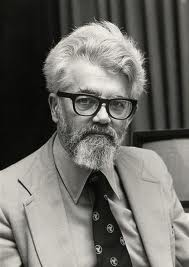
\includegraphics[width=0.8\textwidth]{chap01/10lispauthor}\\
    \tiny John McCarthy    
  \end{minipage}
  \stretchoff
\end{frame}

\begin{frame}[fragile]{发展史}{\texttt{Simula}}
  %\stretchon
  \begin{itemize}
  \item Simula
    \begin{itemize}
    \item 1967
    \item 被认为是第一个面向对象程序设计语言
    \item 第一次引入了对象、数据抽象和类的定义及继承机制
    \item 语法特点\\
      \begin{minipage}{0.8\linewidth}
        \begin{minted}[bgcolor=listinggray, gobble=8, fontsize=\tiny,
          frame=lines]{c++}
          Begin
              Class Char(c);
                  Character c;
                  Begin
                      Procedure print;
                           OutChar(c);
                  End;
          End;
        \end{minted}
      \end{minipage}
    \end{itemize}
  \end{itemize}
  \begin{center}
    \scalebox{0.5}{
      % \tikzstyle{block} = [rectangle, draw, text width=10em, text
      % centered, rounded corners, minimum height=1.0em]
      \tikzset{box/.style={rectangle, draw=black, rounded corners}}
      \tikzset{boxgreen/.style={rectangle, draw=black, rounded corners,fill=green}}
      \begin{tikzpicture}
        \node[box] (asm) {Assembler};
        \node[box] (for) [right=0.5 of asm] {Fortran};
        \node[box] (alg) [right=0.5 of for] {Algol};
        \node[box] (bcp) [right=0.5 of alg] {BCPL};
        \node[box] (pas) [above=1 of bcp] {Pascal};
        \node[boxgreen] (sim) [below=1 of bcp] {Simula};
        \node[box] (c) [right=0.5 of bcp] {C};
        \node[box] (cpp) [right=0.5 of c] {C++};
        \node[box] (cpp0x) [right=0.5 of cpp] {C++0x};
        \node[box] (opas) [above=1 of cpp0x, right=3.1 of pas] {Object Pascal};
        \node[box] (lisp) [below=2.5 of alg] {Lisp};
        \node[box] (smt) [right=2.5 of lisp] {Smalltalk};
        \node[box] (jar) [below=2.5 of cpp0x, right=0.8 of smt] {Java};
        \node (endmain) [right=0.5 of cpp0x] {};
        \node (endopas) [right=0.5 of opas] {};
        \node (endjava) [right=0.5 of jar] {};

        \draw[->] (asm) -- (for);
        \draw[->] (for) -- (alg);
        \draw[->] (alg) -- (bcp);
        \draw[->] ([xshift=0.2em]alg.east) |- (pas);
        \draw[->] ([xshift=0.2em]alg.east) |- (sim);
        \draw[->] (sim.east) -| (cpp);
        % \draw[->] (alg) -- (pas);
        \draw[->] (bcp) -- (c);
        \draw[->] (c) -- (cpp);
        \draw[->] (cpp) -- (cpp0x);
        \draw[->] (cpp0x) -- (endmain);
        \draw[->] ([xshift=0.2em]cpp.east) |- ([yshift=-0.3em]opas.west);
        \draw[->] ([xshift=0.2em]cpp.east) |- ([yshift=0.3em]jar.west);
        \draw[->] (pas) -- (opas);
        \draw[->] (opas) -- (endopas);
        \draw[->] (lisp) -- (smt);
        \draw[->] ([xshift=0.2em]sim.east) |- ([yshift=0.3em]smt.west);
        \draw[->] (smt) -- (jar);
        \draw[->] (jar) -- (endjava);
      \end{tikzpicture}
    }
    \begin{minipage}[b]{0.2\linewidth}
      \centering
      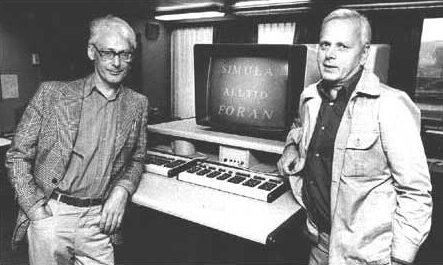
\includegraphics[width=0.8\textwidth]{chap01/11simulaauthor}\\
      \tiny Ole-Johan Dahl and Kristen Nygaard
    \end{minipage}
  \end{center}
  %\stretchoff
\end{frame}

\begin{frame}{发展史}{\texttt{Smalltalk}}
  \begin{itemize}
  \item Smalltalk
    \begin{itemize}
    \item 1972
    \item 第一个纯(Pure)面向对象程序设计语言
    \item 语法特点
      \begin{itemize}
      \item Primitives such as character and punctuation is treated as
        an object\\
        \alert{例如:3+4}\\
        Sends the message “+” to the receiver 3 with argument 4
      \end{itemize}
    \end{itemize}
  \end{itemize}
  \begin{center}
    \scalebox{0.55}{
      % \tikzstyle{block} = [rectangle, draw, text width=10em, text
      % centered, rounded corners, minimum height=1.0em]
      \tikzset{box/.style={rectangle, draw=black, rounded corners}}
      \tikzset{boxgreen/.style={rectangle, draw=black, rounded corners,fill=green}}
      \begin{tikzpicture}
        \node[box] (asm) {Assembler};
        \node[box] (for) [right=0.5 of asm] {Fortran};
        \node[box] (alg) [right=0.5 of for] {Algol};
        \node[box] (bcp) [right=0.5 of alg] {BCPL};
        \node[box] (pas) [above=1 of bcp] {Pascal};
        \node[box] (sim) [below=1 of bcp] {Simula};
        \node[box] (c) [right=0.5 of bcp] {C};
        \node[box] (cpp) [right=0.5 of c] {C++};
        \node[box] (cpp0x) [right=0.5 of cpp] {C++0x};
        \node[box] (opas) [above=1 of cpp0x, right=3.1 of pas] {Object Pascal};
        \node[box] (lisp) [below=2.5 of alg] {Lisp};
        \node[boxgreen] (smt) [right=2.5 of lisp] {Smalltalk};
        \node[box] (jar) [below=2.5 of cpp0x, right=0.8 of smt] {Java};
        \node (endmain) [right=0.5 of cpp0x] {};
        \node (endopas) [right=0.5 of opas] {};
        \node (endjava) [right=0.5 of jar] {};

        \draw[->] (asm) -- (for);
        \draw[->] (for) -- (alg);
        \draw[->] (alg) -- (bcp);
        \draw[->] ([xshift=0.2em]alg.east) |- (pas);
        \draw[->] ([xshift=0.2em]alg.east) |- (sim);
        \draw[->] (sim.east) -| (cpp);
        % \draw[->] (alg) -- (pas);
        \draw[->] (bcp) -- (c);
        \draw[->] (c) -- (cpp);
        \draw[->] (cpp) -- (cpp0x);
        \draw[->] (cpp0x) -- (endmain);
        \draw[->] ([xshift=0.2em]cpp.east) |- ([yshift=-0.3em]opas.west);
        \draw[->] ([xshift=0.2em]cpp.east) |- ([yshift=0.3em]jar.west);
        \draw[->] (pas) -- (opas);
        \draw[->] (opas) -- (endopas);
        \draw[->] (lisp) -- (smt);
        \draw[->] ([xshift=0.2em]sim.east) |- ([yshift=0.3em]smt.west);
        \draw[->] (smt) -- (jar);
        \draw[->] (jar) -- (endjava);
      \end{tikzpicture}
    }
    \begin{minipage}[b]{0.2\linewidth}
      \centering
      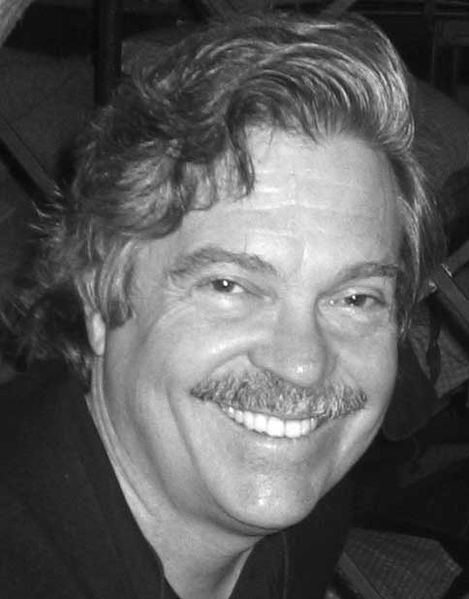
\includegraphics[width=0.8\textwidth]{chap01/12smalltalkauthor}\\
      \tiny Alan Kay
    \end{minipage}
  \end{center}
\end{frame}

\begin{frame}{发展史}{\texttt{C}}
  \begin{itemize}
  \item C
    \begin{itemize}
    \item 1972
    \item C is quirky, flawed, and an enormous success. While
      accidents of history surely helped, it evidently satisfied a
      need for a system implementation language \alert{efficient
        enough to displace assembly language}, yet \alert{sufficiently
        abstract and fluent} to describe algorithms and interactions
      in a wide variety of environments.      
    \end{itemize}
  \end{itemize}
  \begin{center}
    \scalebox{0.55}{
      % \tikzstyle{block} = [rectangle, draw, text width=10em, text
      % centered, rounded corners, minimum height=1.0em]
      \tikzset{box/.style={rectangle, draw=black, rounded corners}}
      \tikzset{boxgreen/.style={rectangle, draw=black, rounded corners,fill=green}}
      \begin{tikzpicture}
        \node[box] (asm) {Assembler};
        \node[box] (for) [right=0.5 of asm] {Fortran};
        \node[box] (alg) [right=0.5 of for] {Algol};
        \node[box] (bcp) [right=0.5 of alg] {BCPL};
        \node[box] (pas) [above=1 of bcp] {Pascal};
        \node[box] (sim) [below=1 of bcp] {Simula};
        \node[boxgreen] (c) [right=0.5 of bcp] {C};
        \node[box] (cpp) [right=0.5 of c] {C++};
        \node[box] (cpp0x) [right=0.5 of cpp] {C++0x};
        \node[box] (opas) [above=1 of cpp0x, right=3.1 of pas] {Object Pascal};
        \node[box] (lisp) [below=2.5 of alg] {Lisp};
        \node[box] (smt) [right=2.5 of lisp] {Smalltalk};
        \node[box] (jar) [below=2.5 of cpp0x, right=0.8 of smt] {Java};
        \node (endmain) [right=0.5 of cpp0x] {};
        \node (endopas) [right=0.5 of opas] {};
        \node (endjava) [right=0.5 of jar] {};

        \draw[->] (asm) -- (for);
        \draw[->] (for) -- (alg);
        \draw[->] (alg) -- (bcp);
        \draw[->] ([xshift=0.2em]alg.east) |- (pas);
        \draw[->] ([xshift=0.2em]alg.east) |- (sim);
        \draw[->] (sim.east) -| (cpp);
        % \draw[->] (alg) -- (pas);
        \draw[->] (bcp) -- (c);
        \draw[->] (c) -- (cpp);
        \draw[->] (cpp) -- (cpp0x);
        \draw[->] (cpp0x) -- (endmain);
        \draw[->] ([xshift=0.2em]cpp.east) |- ([yshift=-0.3em]opas.west);
        \draw[->] ([xshift=0.2em]cpp.east) |- ([yshift=0.3em]jar.west);
        \draw[->] (pas) -- (opas);
        \draw[->] (opas) -- (endopas);
        \draw[->] (lisp) -- (smt);
        \draw[->] ([xshift=0.2em]sim.east) |- ([yshift=0.3em]smt.west);
        \draw[->] (smt) -- (jar);
        \draw[->] (jar) -- (endjava);
      \end{tikzpicture}
    }
    \begin{minipage}[b]{0.2\linewidth}
      \centering
      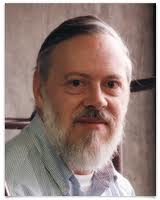
\includegraphics[width=0.8\textwidth]{chap01/13cauthor}\\
      \tiny Dennis Ritchie
    \end{minipage}
  \end{center}
\end{frame}

\begin{frame}{发展史}{\texttt{C++}}
  \begin{itemize}
  \item C++
    \begin{itemize}
    \item 1985 
    \end{itemize}
  \end{itemize}
  \begin{center}
    \scalebox{0.65}{
      % \tikzstyle{block} = [rectangle, draw, text width=10em, text
      % centered, rounded corners, minimum height=1.0em]
      \tikzset{box/.style={rectangle, draw=black, rounded corners}}
      \tikzset{boxgreen/.style={rectangle, draw=black, rounded corners,fill=green}}
      \begin{tikzpicture}
        \node[box] (asm) {Assembler};
        \node[box] (for) [right=0.5 of asm] {Fortran};
        \node[box] (alg) [right=0.5 of for] {Algol};
        \node[box] (bcp) [right=0.5 of alg] {BCPL};
        \node[box] (pas) [above=1 of bcp] {Pascal};
        \node[box] (sim) [below=1 of bcp] {Simula};
        \node[box] (c) [right=0.5 of bcp] {C};
        \node[boxgreen] (cpp) [right=0.5 of c] {C++};
        \node[box] (cpp0x) [right=0.5 of cpp] {C++0x};
        \node[box] (opas) [above=1 of cpp0x, right=3.1 of pas] {Object Pascal};
        \node[box] (lisp) [below=2.5 of alg] {Lisp};
        \node[box] (smt) [right=2.5 of lisp] {Smalltalk};
        \node[box] (jar) [below=2.5 of cpp0x, right=0.8 of smt] {Java};
        \node (endmain) [right=0.5 of cpp0x] {};
        \node (endopas) [right=0.5 of opas] {};
        \node (endjava) [right=0.5 of jar] {};

        \draw[->] (asm) -- (for);
        \draw[->] (for) -- (alg);
        \draw[->] (alg) -- (bcp);
        \draw[->] ([xshift=0.2em]alg.east) |- (pas);
        \draw[->] ([xshift=0.2em]alg.east) |- (sim);
        \draw[->] (sim.east) -| (cpp);
        % \draw[->] (alg) -- (pas);
        \draw[->] (bcp) -- (c);
        \draw[->] (c) -- (cpp);
        \draw[->] (cpp) -- (cpp0x);
        \draw[->] (cpp0x) -- (endmain);
        \draw[->] ([xshift=0.2em]cpp.east) |- ([yshift=-0.3em]opas.west);
        \draw[->] ([xshift=0.2em]cpp.east) |- ([yshift=0.3em]jar.west);
        \draw[->] (pas) -- (opas);
        \draw[->] (opas) -- (endopas);
        \draw[->] (lisp) -- (smt);
        \draw[->] ([xshift=0.2em]sim.east) |- ([yshift=0.3em]smt.west);
        \draw[->] (smt) -- (jar);
        \draw[->] (jar) -- (endjava);
      \end{tikzpicture}
    }
    \begin{minipage}[b]{0.2\linewidth}
      \centering
      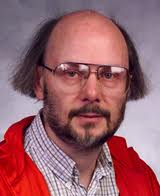
\includegraphics[width=1.0\textwidth]{chap01/14cppauthor}\\
      \tiny Bjarne Stroustrup \\ (本贾尼·斯特劳斯特卢普)
    \end{minipage}
  \end{center}
\end{frame}

\begin{frame}{发展史}{\texttt{JAVA}}
  \begin{itemize}
  \item JAVA
    \begin{itemize}
    \item 1995 
    \end{itemize}
  \end{itemize}
  \begin{center}
    \scalebox{0.7}{
      % \tikzstyle{block} = [rectangle, draw, text width=10em, text
      % centered, rounded corners, minimum height=1.0em]
      \tikzset{box/.style={rectangle, draw=black, rounded corners}}
      \tikzset{boxgreen/.style={rectangle, draw=black, rounded corners,fill=green}}
      \begin{tikzpicture}
        \node[box] (asm) {Assembler};
        \node[box] (for) [right=0.5 of asm] {Fortran};
        \node[box] (alg) [right=0.5 of for] {Algol};
        \node[box] (bcp) [right=0.5 of alg] {BCPL};
        \node[box] (pas) [above=1 of bcp] {Pascal};
        \node[box] (sim) [below=1 of bcp] {Simula};
        \node[box] (c) [right=0.5 of bcp] {C};
        \node[box] (cpp) [right=0.5 of c] {C++};
        \node[box] (cpp0x) [right=0.5 of cpp] {C++0x};
        \node[box] (opas) [above=1 of cpp0x, right=3.1 of pas] {Object Pascal};
        \node[box] (lisp) [below=2.5 of alg] {Lisp};
        \node[box] (smt) [right=2.5 of lisp] {Smalltalk};
        \node[boxgreen] (jar) [below=2.5 of cpp0x, right=0.8 of smt] {Java};
        \node (endmain) [right=0.5 of cpp0x] {};
        \node (endopas) [right=0.5 of opas] {};
        \node (endjava) [right=0.5 of jar] {};

        \draw[->] (asm) -- (for);
        \draw[->] (for) -- (alg);
        \draw[->] (alg) -- (bcp);
        \draw[->] ([xshift=0.2em]alg.east) |- (pas);
        \draw[->] ([xshift=0.2em]alg.east) |- (sim);
        \draw[->] (sim.east) -| (cpp);
        % \draw[->] (alg) -- (pas);
        \draw[->] (bcp) -- (c);
        \draw[->] (c) -- (cpp);
        \draw[->] (cpp) -- (cpp0x);
        \draw[->] (cpp0x) -- (endmain);
        \draw[->] ([xshift=0.2em]cpp.east) |- ([yshift=-0.3em]opas.west);
        \draw[->] ([xshift=0.2em]cpp.east) |- ([yshift=0.3em]jar.west);
        \draw[->] (pas) -- (opas);
        \draw[->] (opas) -- (endopas);
        \draw[->] (lisp) -- (smt);
        \draw[->] ([xshift=0.2em]sim.east) |- ([yshift=0.3em]smt.west);
        \draw[->] (smt) -- (jar);
        \draw[->] (jar) -- (endjava);
      \end{tikzpicture}
    }
    \begin{minipage}[b]{0.2\linewidth}
      \centering
      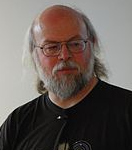
\includegraphics[width=0.8\textwidth]{chap01/15javaauthor}\\
      \tiny James Gosling
    \end{minipage}
  \end{center}
\end{frame}

%%%%%%%%%%%%%%%%%%%%%%%%%%%%%%%%%%%%%%%%%%%%%%%%%%%%%%%%%%%%%%%%%%%%%%%%%%

\section[目的]{为何使用C++实践面向对象程序设计}\label{sec:chap01-sec05}

%%%%%%%%%%%%%%%%%%%%%%%%%% 为何使用C++实践面向对象程序设计 %%%%%%%%%%%%%%%%%%%%%%%%%%%%%
\begin{frame}{目的}{面向对象程序设计}
  \stretchon
  \begin{itemize}
  \item Java\\
    网络计算(Network computing)
  \item C++\\
    系统程序设计(Systems programming)\\
    \begin{center}
      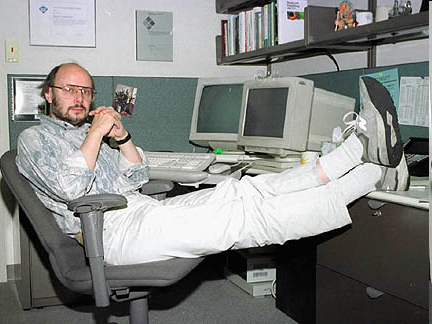
\includegraphics[width=0.4\textwidth]{chap01/16cppauthor2}\\
      \tiny Bjarne Stroustrup\\
      \url{http://www2.research.att.com/~bs/}
    \end{center}    
  \end{itemize}
  \stretchoff
\end{frame}

\begin{frame}{目的}{C++应用程序开发案例}
  \stretchon
  \begin{itemize}
  \item Adobe系统:Photoshop, Illustrator等
  \item Alias|Wavefront: Maya, Autodesk等
  \item Apple OS X重要的部分
  \item 游戏: 星际争霸,暗黑破坏神,魔兽争霸等
  \item Telecommunications
  \item Google(网络搜索引擎等)
  \item Microsoft applications and GUIs
  \item Linux tools and GUIs
  \item Amazon.com: 大型电子商务应用软件
  \item \ldots\ldots
  \end{itemize}
  \stretchoff
\end{frame}

\begin{frame}{目的}{为后续课程做准备}
  \stretchon
  \begin{itemize}
  \item Java 、C\#和Objective C
  \item 计算机图形学及计算机动画
  \item 图形图像处理
  \item 虚拟现实技术
  \item \ldots\ldots
  \end{itemize}
  \stretchoff
\end{frame}
%%%%%%%%%%%%%%%%%%%%%%%%%%%%%%%%%%%%%%%%%%%%%%%%%%%%%%%%%%%%%%%%%%%%%%%%%%

\section[程序结构]{C++程序结构}\label{sec:chap01-sec06}
%%%%%%%%%%%%%%%%%%%%%%%%%%%%%%%% C++程序结构 %%%%%%%%%%%%%%%%%%%%%%%%%%%%%%%%%%
\begin{frame}{程序结构}{C++程序结构}
  \stretchon
  \begin{itemize}
  \item 开发流程
  \end{itemize}
  % \scalebox{0.7}{
  \centering
  %\begin{center}
    \scalebox{0.95}{
    $%
    \psset{shadowcolor=black!70,shadowangle=-90,blur,shortput=nab}
    \begin{psmatrix}[rowsep=0.5,colsep=1.7]
      \psframebox[fillstyle=solid,
      fillcolor=green!30,shadow=true]{\text{编译器}} &
      \psframebox[fillstyle=solid, fillcolor=gray!30,shadow=true]{
        \begin{minipage}[c]{0.25\linewidth}
          \text{源程序.cpp}\\
          \text{头文件.h}\\
          \textcolor{red}{系统头文件}
        \end{minipage}
      }\\
      \psframebox[fillstyle=solid,
      fillcolor=yellow!30,shadow=true]{\text{预处理器}} &
      \psframebox[fillstyle=solid,
      fillcolor=gray!30,shadow=true]{\text{源程序.cpp}}\\
      \psframebox[fillstyle=solid,
      fillcolor=yellow!30,shadow=true]{\text{编译器}} &
      \psframebox[fillstyle=solid, fillcolor=gray!30,shadow=true]{
        \begin{minipage}[c]{0.25\linewidth}
          \text{目标程序.obj}\\
          \text{库文件.lib}
        \end{minipage}
      }
      & \psframebox[fillstyle=solid, fillcolor=red!30,shadow=true]{\text{调试器}} \\
      \psframebox[shadow=true]{\text{连接器}} &
      \psframebox[fillstyle=solid,
      fillcolor=gray!30,shadow=true]{\text{可执行文件.exe}}\\
      \psframebox[fillstyle=solid,
      fillcolor=red!30,shadow=true]{\text{CPU}} &
      \psframebox[shadow=true]{\text{内存}}
      \psset{arrows=->,nodesep=3pt}
      \everypsbox{\scriptstyle}
      \ncline{1,1}{2,1}
      \ncline{2,1}{3,1}
      \ncline{3,1}{4,1}
      \ncline{4,1}{5,1}
      \ncline{<->}{1,1}{1,2}^{\text{\textcolor{red}{编辑}}}
      \ncline{1,2}{2,1}
      \ncline{2,1}{2,2}^{\text{\textcolor{red}{预处理}}}
      \ncline{2,2}{3,1}
      \ncline{3,1}{3,2}^{\text{\textcolor{red}{编译}}}
      \ncline{3,2}{4,1}
      \ncline{4,1}{4,2}^{\text{\textcolor{red}{连接}}}
      \ncline{4,2}{5,2}>{\text{\textcolor{red}{载入}}}
      \ncline{5,1}{5,2}^{\text{\textcolor{red}{运行}}}
      \ncangle[angleA=90,angleB=0, armB=0, linearc=0]{3,3}{1,2}>{\text{\textcolor{red}{调试}}}
      \ncangle[angleA=-90,angleB=0, armB=0, linearc=0]{3,3}{5,2}>{\text{\textcolor{red}{调试}}}
    \end{psmatrix}
    $%
    }
    % \end{center}
  \stretchoff  
\end{frame}

\begin{frame}{程序结构}{集成开发环境---IDE}
  \stretchon
  \begin{itemize}
  \item 辅助程序
  \item 工具
    \begin{itemize}
    \item 编辑器
    \item 编译器/解释器
    \item 自动建立工具
    \item 调试器
    \item 版本控制器
    \item GUI设计器
    \item \ldots\ldots
    \end{itemize}
  \end{itemize}
  \stretchoff
\end{frame}

\begin{frame}{程序结构}{IDE---DEV C++}
  \stretchon
  \begin{itemize}
  \item DEV C++
  \end{itemize}
  \centering
  %\begin{center}
    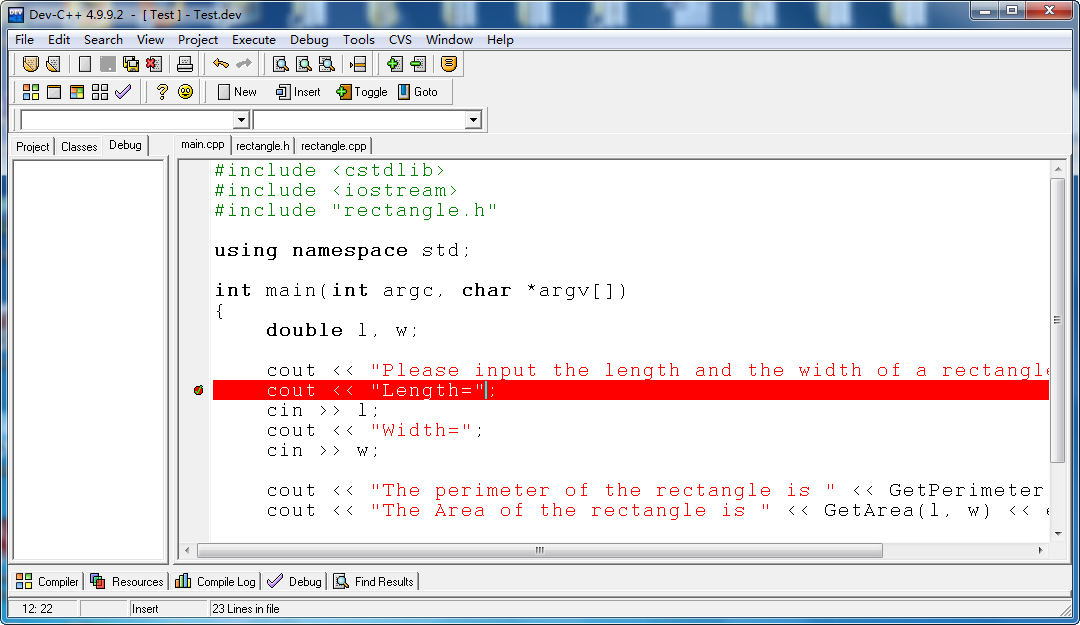
\includegraphics[height=0.6\textheight]{chap01/17idedevc}\\
    \tiny
    \url{http://sourceforge.net/projects/orwelldevcpp/}
    % \end{center}
  \stretchoff
\end{frame}

\begin{frame}{程序结构}{IDE---Visual Studio 2005}
  \stretchon
  \begin{itemize}
  \item Visual Studio 2005
  \end{itemize}
  \centering
  %\begin{center}
    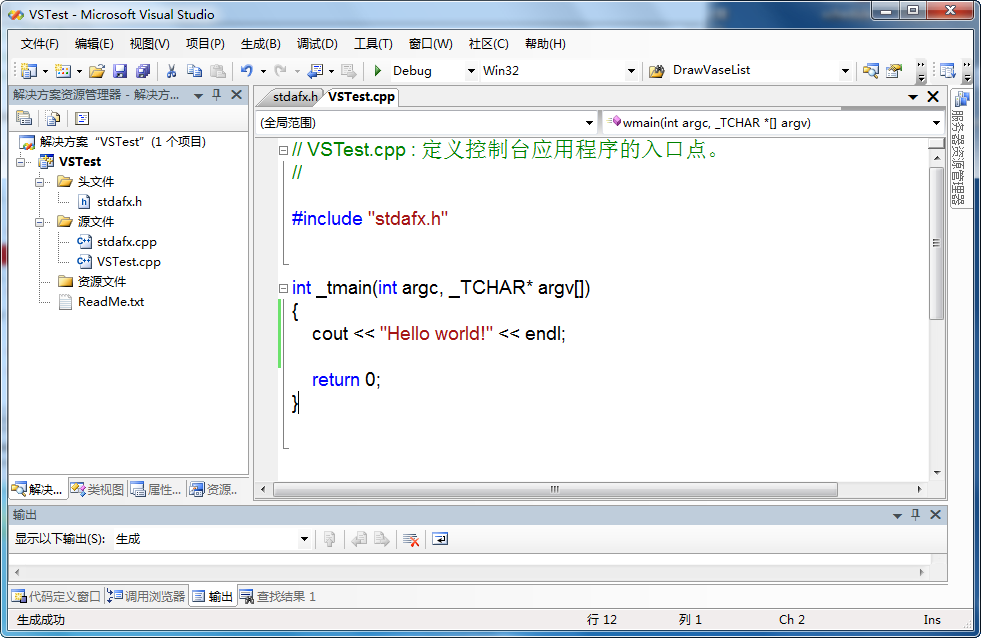
\includegraphics[height=0.6\textheight]{chap01/18idevs2005}\\
    \tiny
    \url{http://www.visualstudio.com/}
  %\end{center}
  \stretchoff
\end{frame}

\begin{frame}{程序结构}{IDE---Code::Blocks}
  \stretchon
  \begin{itemize}
  \item Code::Blocks
  \end{itemize}
  \centering
  %\begin{center}
    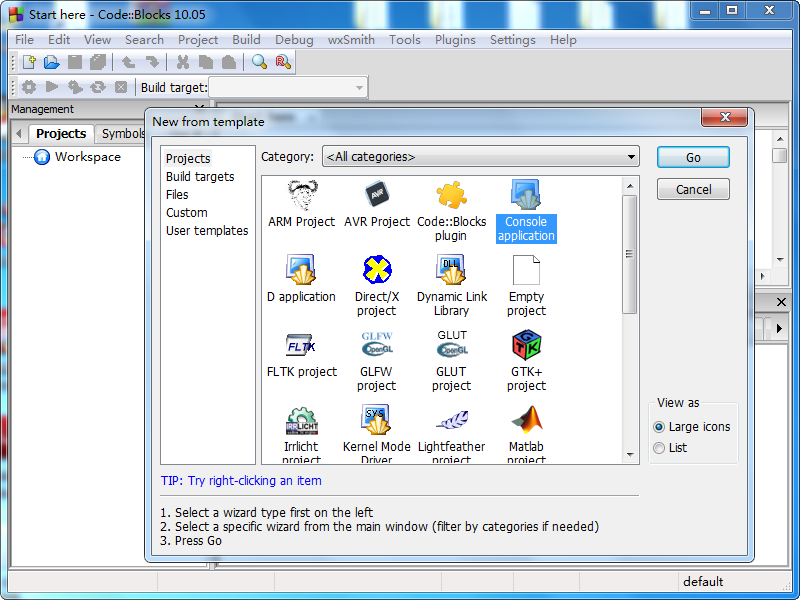
\includegraphics[height=0.6\textheight]{chap01/19idecb}\\
    \tiny
    \url{http://www.codeblocks.org/}
  %\end{center}
  \stretchoff
\end{frame}

\begin{frame}{程序结构}{IDE---QT}
  \stretchon
  \begin{itemize}
  \item QT
  \end{itemize}
  \centering
  %\begin{center}
    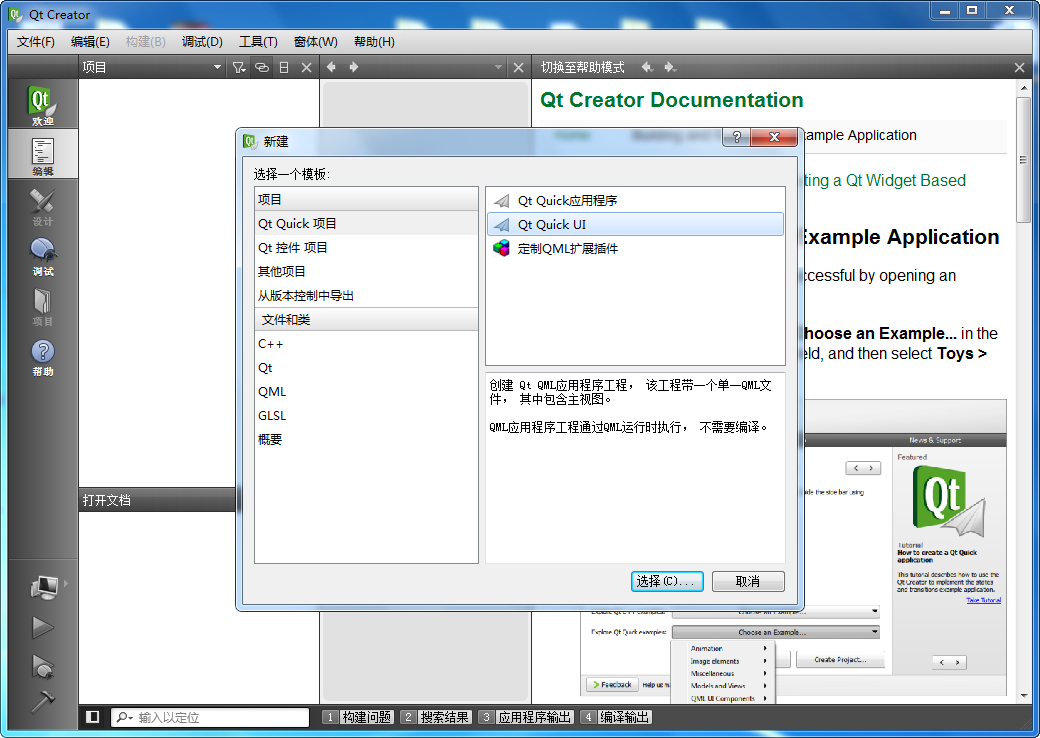
\includegraphics[height=0.6\textheight]{chap01/20ideqt}\\
    \tiny
    \url{http://qt-project.org/}
  %\end{center}
  \stretchoff
\end{frame}
  
  
%%%%%%%%%%%%%%%%%%%%%%%%%%%%%%%%%%%%%%%%%%%%%%%%%%%%%%%%%%%%%%%%%%%%%%%%%%


\section[基本程序]{基本C++程序}\label{sec:chap01-sec07}
%%%%%%%%%%%%%%%%%%%%%%%%%%%%%%%% 基本C++程序 %%%%%%%%%%%%%%%%%%%%%%%%%%%%%%%%%%
\begin{frame}[fragile]{基本程序}{基本C++程序}
  \vspace{-2ex}
  \begin{center}
    \begin{minipage}{0.8\linewidth}
      \cppfile{codes/chap01/ex01-01.cpp}
    \end{minipage}
  \end{center}
  \vspace{-4ex}
  \begin{itemize}
  \item 名字空间 (namespace)\\
    \begin{minipage}{0.8\linewidth}
      \begin{cppcode}
using namespace std;
      \end{cppcode}
    \end{minipage}
  \item 输入/输出
    \begin{itemize}
    \item cin对象\\
      \begin{minipage}{0.8\linewidth}
      \begin{cpptt}
cin >> |对象1| >> |对象2| >> |$\cdots$| >> |对象n|;
      \end{cpptt}
    \end{minipage}
  \item cout对象\\
    \begin{minipage}{0.8\linewidth}
      \begin{cpptt}
cout << |对象1| << |对象2| << |$\cdots$| << |对象n|;
      \end{cpptt}
    \end{minipage}
    \end{itemize}
  \end{itemize}
\end{frame}

\begin{frame}[fragile]{基本程序}{基本C++程序}%label=testframe,
  %\begin{spacing}{1.2}
  \begin{itemize}
  \item 两个整数的加法       
  \end{itemize}
  \begin{center}
    \begin{tikzpicture}[font=\scriptsize]
      % 绘制代码
      \umlnote[scale=0.95, text width=0.65\textwidth](code1) at (0, 0)
      {
        \cppfile{codes/chap01/ex01-02.cpp}
      };
    \end{tikzpicture}
  \end{center}
  %\end{spacing}
\end{frame}
%%%%%%%%%%%%%%%%%%%%%%%%%%%%%%%%%%%%%%%%%%%%%%%%%%%%%%%%%%%%%%%%%%%%%%%%%%

% 附件页
\section[附件下载]{本讲示例代码及附件下载} 
\begin{frame}[t]{附件}{本讲附件}
  % 此处的[ucfilespec=...]必须指定为pdf否则Windows下无法下载
  %\vspace{-4ex}
  \textattachfile[ucfilespec=ex-src01.pdf]{ex-src01.zip}{附件:右键单击该
    链接,选择\qtmark{\alert{保存附件}}下载,\alert{将后缀名改为\qtmark{.zip}解压}
      \footnote[frame]{请\alert{退出全屏模式}后点击该链接。}
      \footnote[frame]{以Adobe Acrobat Reader为例。}
      。}%\\

  \vspace{-1ex}
  \begin{center}
    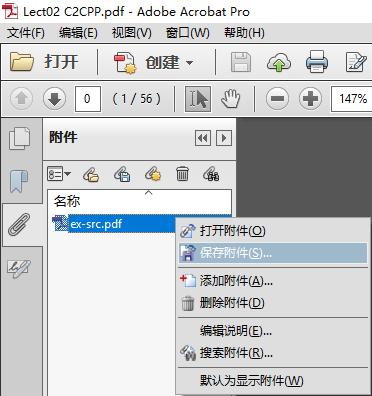
\includegraphics[height=0.35\textheight]{pdfattatchdownload01}\quad
    %或 \quad%
    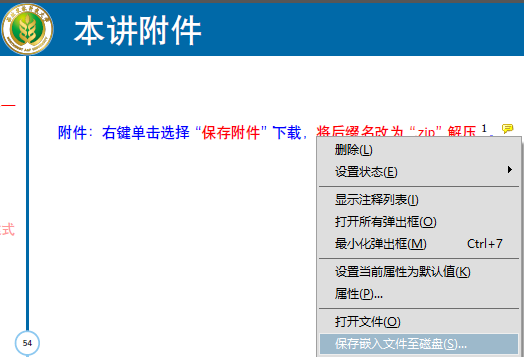
\includegraphics[height=0.35\textheight]{pdfattatchdownload02}\\[2ex]%
    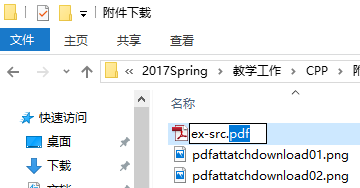
\includegraphics[height=0.255\textheight]{pdfattatchdownload03}\quad
    %$\Rightarrow$ \quad%
    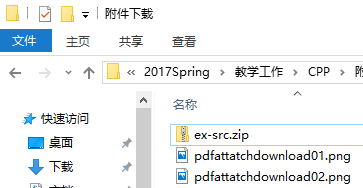
\includegraphics[height=0.255\textheight]{pdfattatchdownload04}%
  \end{center}   
\end{frame}

% \tiny
% \scriptsize
% \footnotesize
% \small
% \normalsize
% \large
% \Large
% \LARGE
% \huge
% \Huge


%%% Local Variables: 
%%% mode: latex
%%% TeX-master: "../main.tex"
%%% End: 
